\mychapter{System Integration}{System Integration}{}
\label{chap:sysInt}


\mysection{System Diagram}{System Diagram}

\begin{figure}[H]
    \centering
    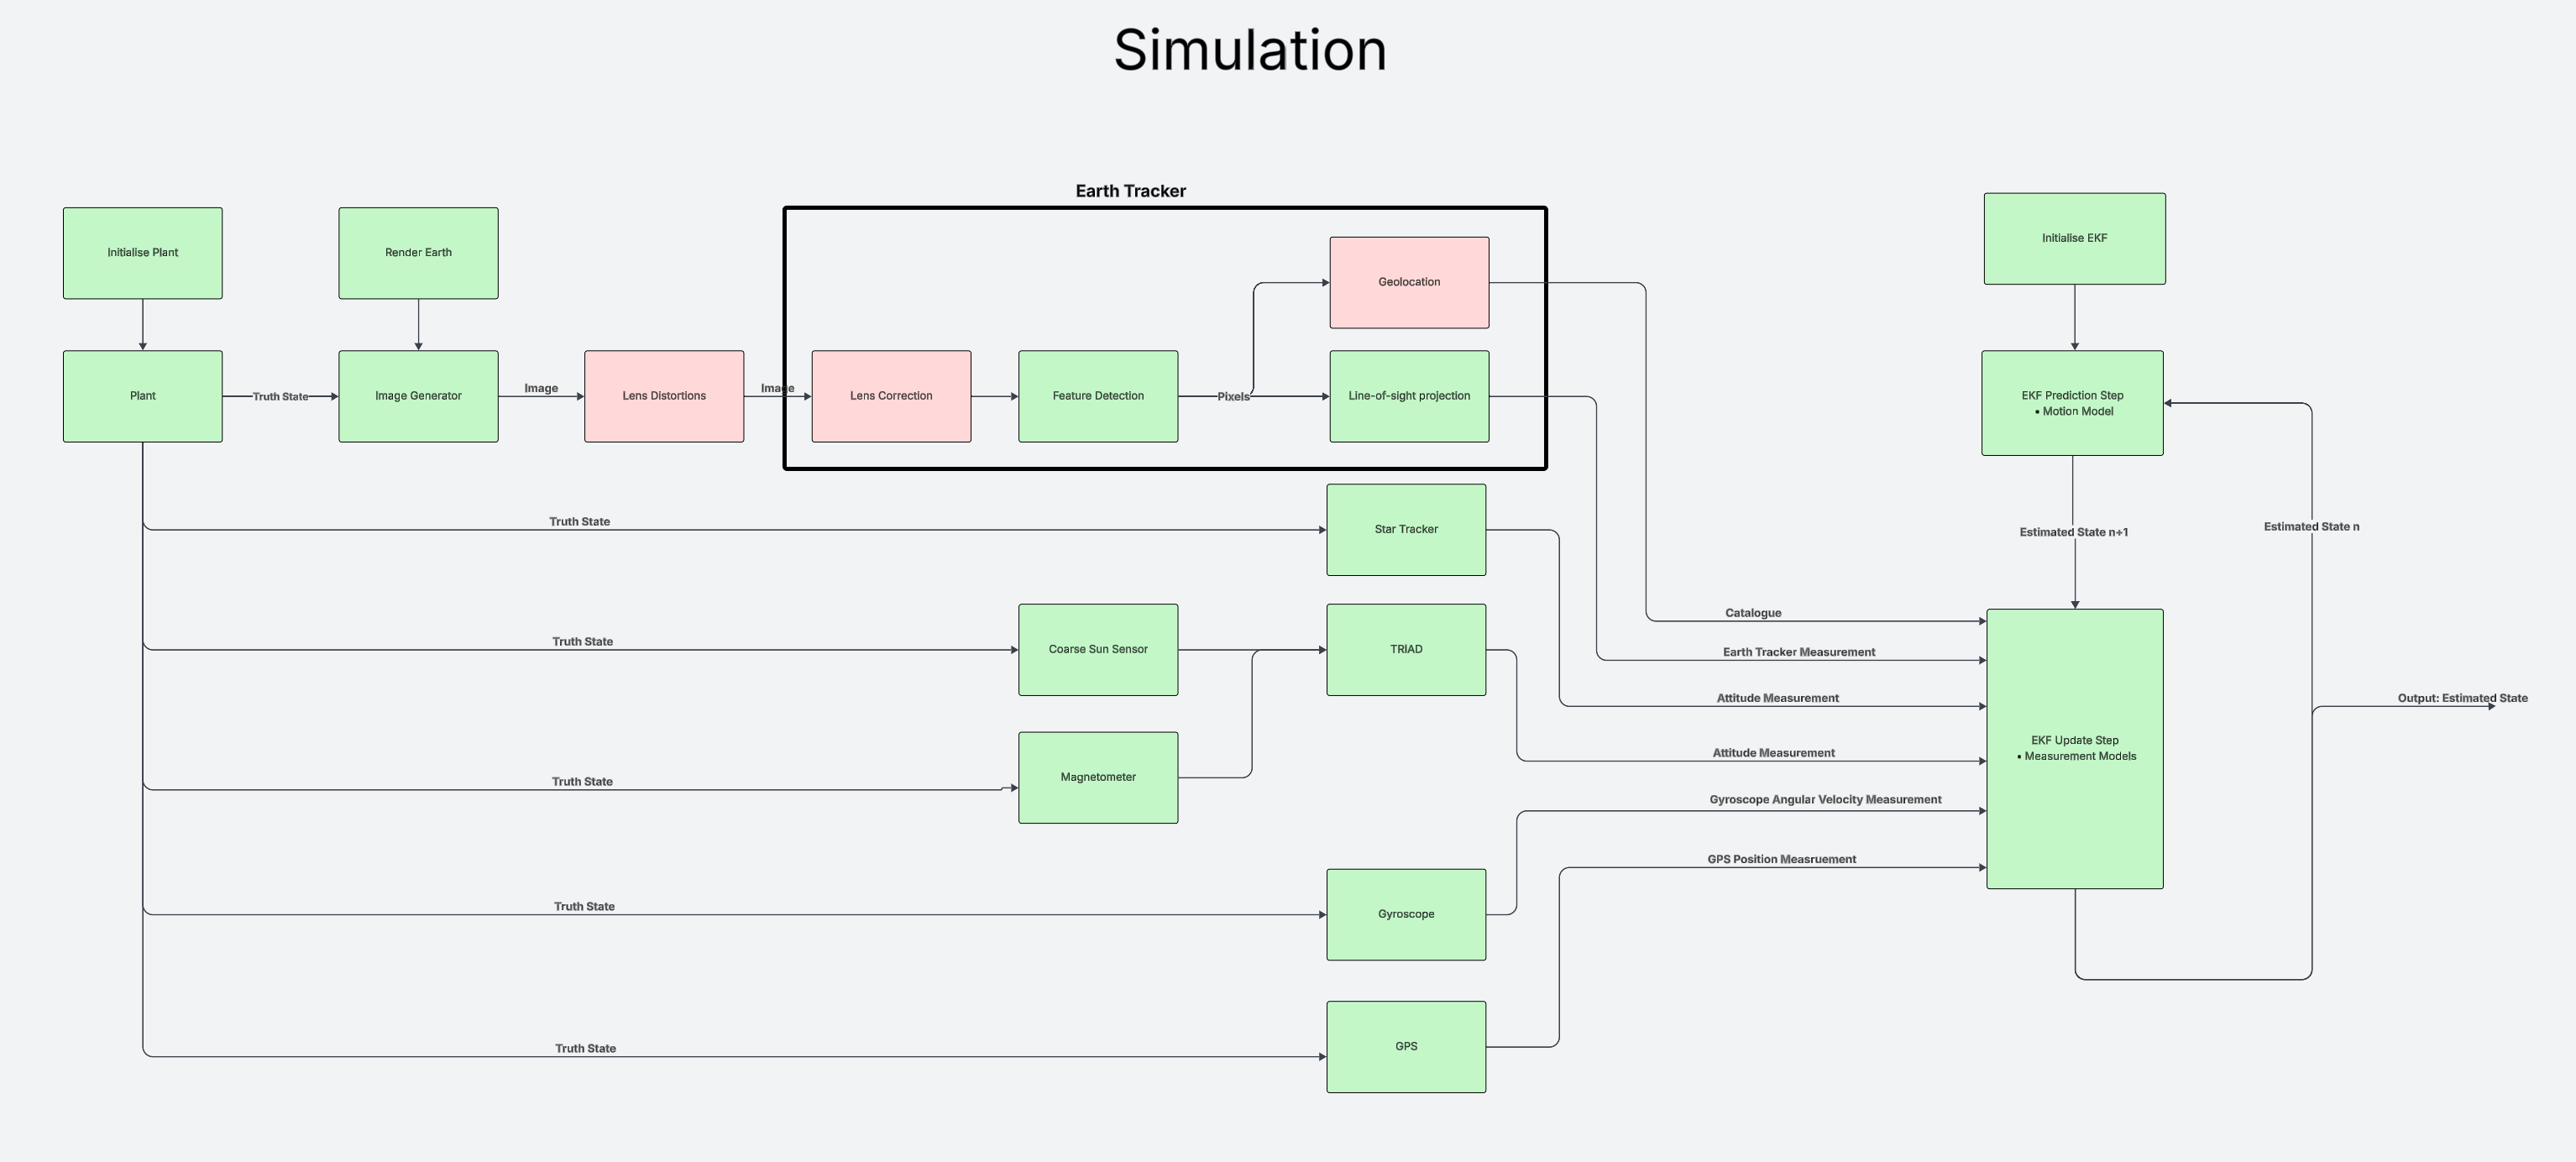
\includegraphics[width=1\linewidth]{figures/SystemIntegration/FullSystemDiagram.png}
    \caption{Image Plane}
    \label{fig4.2}
\end{figure}

\mysection{System Initialization}{System Initialization}

The orbital system is initialized using the following parameters:

\begin{itemize}
    \item \textbf{Latitude}: Initial geodetic latitude of the satellite.
    \item \textbf{Longitude}: Initial geodetic longitude of the satellite.
    \item \textbf{Altitude}: Initial altitude above the WGS84 ellipsoid.
    \item \textbf{Roll (X-axis)}: Initial roll angle of the satellite body with respect to the orbital reference frame.
    \item \textbf{Pitch (Y-axis)}: Initial pitch angle of the satellite body with respect to the orbital reference frame.
    \item \textbf{Yaw (Z-axis)}: Initial yaw angle of the satellite body with respect to the orbital reference frame.
\end{itemize}

The geodetic latitude, longitude, and altitude are first converted to an inertial position vector using the WGS84 Earth model. This involves a transformation from the local geodetic frame to the Earth-Centered Earth-Fixed (ECEF) frame, followed by a rotation into the inertial frame:

\begin{equation}
    \mathbf{r}_\mathcal{I} = T_\mathcal{R}^\mathcal{I} \left( T_\mathcal{L}^{\mathcal{R}}(\mathbf{r}_\mathcal{L}, \omega_e, t) \right)
\end{equation}

To compute the initial velocity vector, it is assumed that the satellite is in a near-circular orbit, and thus its velocity vector is orthogonal to its position vector. While multiple solutions satisfy this constraint, the velocity direction is resolved using the local east unit vector, which is always tangential to the satellite’s position on the Earth's surface. The eastward direction is given by:

\begin{equation}
    \mathbf{u}_{\text{east}} = \frac{1}{|| \cdot ||} \begin{bmatrix}
        -\sin(\lambda) \\
        \cos(\lambda) \\
        0
    \end{bmatrix}
\end{equation}

where \( \lambda \) is the geodetic longitude. The vector is normalized to obtain a unit direction.

The magnitude of the orbital velocity is computed using the vis-viva equation:

\begin{equation}
    \left|| \mathbf{v} \right|| = \sqrt{\frac{\mu}{\left|| \mathbf{r} \right||}}
\end{equation}

where \( \mu \) is the standard gravitational parameter, and \( \left|| \mathbf{r} \right|| \) is the norm of the inertial position vector.

The inertial velocity vector is then calculated as:

\begin{equation}
    \mathbf{v}_\mathcal{I} = \left|| \mathbf{v} \right|| \cdot \mathbf{u}_{\text{east}}
\end{equation}

\textcolor{blue}{Add some pictures for visualisation}


The satellite's initial attitude is defined by two sequential quaternion rotations:

\begin{itemize}
    \item \( q_{\mathcal{O}/\mathcal{I}} \): the quaternion representing the rotation from the inertial (ECI) frame \( \mathcal{I} \) to the orbital reference frame \( \mathcal{O} \),
    \item \( q_{\mathcal{B}/\mathcal{O}} \): the quaternion representing the rotation from the orbital frame \( \mathcal{O} \) to the satellite body frame \( \mathcal{B} \),
\end{itemize}

These quaternions are constructed using the initial orbital position (from latitude, longitude, and altitude) and the initial roll, pitch, and yaw of the satellite body with respect to the orbital frame. 

The total attitude of the satellite body with respect to the inertial frame is given by the quaternion composition:

\begin{equation}
    q_{\mathcal{B}/\mathcal{I}} = q_{\mathcal{B}/\mathcal{O}} \otimes q_{\mathcal{O}/\mathcal{I}}
\end{equation}

where \( \otimes \) denotes quaternion multiplication, performed right-to-left (i.e., the rotation \( q_{\mathcal{O}/\mathcal{I}} \) is applied first, followed by \( q_{\mathcal{B}/\mathcal{O}} \)).

\paragraph{Reference Frame Alignment at Initialization}

At the simulation start time \( t = 0 \), it is assumed that the Earth-Centered, Earth-Fixed (ECEF) frame \( \mathcal{R} \) is aligned with the inertial frame \( \mathcal{I} \). This is a common simplification used in orbital mechanics when time is initialized at a known Greenwich Mean Sidereal Time (GMST), typically zero. This alignment implies:

\begin{equation}
    R_\mathcal{R}^\mathcal{I}(t=0) = \mathbf{I}_{3 \times 3}
\end{equation}

where \( R_\mathcal{R}^\mathcal{I} \) is the rotation matrix from ECEF to ECI. This simplifies the initial attitude calculations and ensures consistent initialization across reference frames.

\paragraph{Angular Velocity Initialization}

The initial angular velocity of the satellite body is specified relative to the orbital frame:

\begin{equation}
    \boldsymbol{\omega}_{\mathcal{B/O}}^{\mathcal{B}} = 
    \begin{bmatrix}
        \omega_x \\
        \omega_y \\
        \omega_z
    \end{bmatrix}
\end{equation}

Since the ECI and ECEF frames are aligned at \( t = 0 \), and the orbital frame is defined in the ECI frame, this implies that the angular velocity of the body with respect to the inertial frame is initially equivalent to the angular velocity with respect to the orbital frame:

\begin{equation}
    \boldsymbol{\omega}_{\mathcal{B/I}}^{\mathcal{B}}(t = 0) = \boldsymbol{\omega}_{\mathcal{B/O}}^{\mathcal{B}}(t = 0)
\end{equation}

This relationship holds only at the initialization instant. As time progresses, the orbital frame rotates relative to the inertial frame due to the satellite's motion, and the distinction between \( \boldsymbol{\omega}_{\mathcal{B/I}} \) and \( \boldsymbol{\omega}_{\mathcal{B/O}} \) becomes significant and must be handled accordingly in the attitude propagation.
